\section{Failure-Mode Taxonomy}
\label{app:taxonomy}

\subsection{Labeling procedure}

After the audit a language model reads each run's event transcript, its final report, and
the audit verdict, rationale, and flags, and gives the run one primary
failure mode. A run can show more than one mechanism, so the label names the
dominant one, and labeling never changes a score, verdict, or flag. We add a
new mode only when at least two runs show it. The taxonomy has nine modes with
fixed names (Table~\ref{tab:taxonomy}). Before pooling the sweeps we mapped
retired names, underscore spellings, and sweep-local labels onto the nine.
Thirty-six runs had a label outside that vocabulary or one that contradicted
the pinned verdict, and we re-read them against the definitions and relabeled
them from what the agent did. The labels folded this way are
under-determined-target, scope-collapse, unavailability-concluded-from-prose,
context-or-round-exhaustion, fabrication and fabrication-or-provenance-break,
report-serialization-fault and report-serialization-collapse,
tool-call-format-collapse, protocol-drift-direction-flip,
eval-protocol-shopping, verified-non-attempt, and success. Ten of the 36
had a valid label that disagreed with the pinned verdict, and seven of those
ten were labeled near-miss-partial on a disqualified run. We kept the label on
four runs, three of them from inside that seven, where the only high-severity
flag concerned the run's self-report. The fourth is outside the seven, and we
kept it as a provenance mismatch because the dissection found its passing value
was measured on a sibling checkpoint the dataset row does not pin.
Figure~\ref{fig:failure-modes} and Table~\ref{tab:failure-modes-by-agent} use
the plain-language names under the slugs in Table~\ref{tab:taxonomy}, in the
same order.

\begin{table}[t]
\centering
\fontsize{8}{9.6}\selectfont
\setlength{\tabcolsep}{3.5pt}
\begin{tabular}{@{}lccccc@{}}
\toprule
Mode & DeepSeek-V4-Flash & Qwen3.6-27B & MiniMax-M2.7 & Muse Spark 1.2 & All \\
\midrule
Reproduced & 27 & 13 & 10 & 22 & 72 \\
Ran, outside tolerance & 26 & 16 & 7 & 27 & 76 \\
Reimplemented but did not check the result & 13 & 16 & 27 & 7 & 63 \\
Build and dependency failures & 1 & 8 & 11 & 4 & 24 \\
Wrong artifact measured & 6 & 4 & 13 & 15 & 38 \\
Wrong experiment & 9 & 11 & 16 & 10 & 46 \\
Echoed a shipped number & 1 & 1 & 4 & 3 & 9 \\
Never launched an experiment & 2 & 2 & 4 & 5 & 13 \\
Failed before any number was produced & 2 & 19 & 6 & 4 & 31 \\
No label & 13 & 10 & 2 & 3 & 28 \\
\midrule
Cells & 100 & 100 & 100 & 100 & 400 \\
\bottomrule
\end{tabular}
\caption{Primary failure mode by agent.}
\label{tab:failure-modes-by-agent}
\end{table}

\subsection{The failure modes}

The rubric anchor column of Table~\ref{tab:taxonomy} names the band of the
frozen rubric in Appendix~\ref{app:rubric} whose conditions match the mode's
evidence signature. Because the auditor never sees the mode label and grades
each run from that run's own evidence, observed scores spread around the
anchor.

\begingroup
\footnotesize
\begin{longtable}{@{}>{\raggedright\arraybackslash}p{3.05cm}>{\raggedright\arraybackslash}p{3.85cm}>{\raggedright\arraybackslash}p{3.65cm}>{\raggedright\arraybackslash}p{1.6cm}@{}}
\toprule
Mode & Definition & Evidence signature & Rubric anchor \\
\midrule
\endfirsthead
\multicolumn{4}{@{}l}{\footnotesize\itshape Table~\ref{tab:taxonomy}, continued.} \\[3pt]
\toprule
Mode & Definition & Evidence signature & Rubric anchor \\
\midrule
\endhead
\midrule
\endfoot
\bottomrule
\noalign{\vskip 6pt}
\caption{The nine failure modes, one primary mode per run. The rubric anchor is
the band whose conditions match the mode's evidence signature, and scores spread
around it.}
\label{tab:taxonomy}\\
\endlastfoot
\texttt{reproduced-\allowbreak clean}\newline \emph{Reproduced} &
The agent runs the pinned experiment, using the released artifacts the tier provides, and the
graded number lands inside the pinned bar. &
A number the run computed, traced to a command in the transcript that ran
the experiment on the released artifacts the tier provides. &
8--10 \\
\addlinespace
\texttt{near-\allowbreak miss-\allowbreak partial}\newline \emph{Ran, outside tolerance} &
The agent runs the right pipeline and measures a number that misses the bar. &
A completed run of the pinned quantity with clean provenance, and a measured
value on the wrong side of the bar. &
6--7 \\
\addlinespace
\texttt{reimplement-\allowbreak without-\allowbreak validating}\newline \emph{Reimplemented but did not check the result} &
The agent writes its own version of the method, or part of it, and never
checks any stage against a reference it did not produce. &
A component written from scratch in the run's own code, and a reference
number the paper supplies, most often its baseline in the same table as the
target, that the transcript never compares against. &
4 \\
\addlinespace
\texttt{environment-\allowbreak fights}\newline \emph{Build and dependency failures} &
Most of the run goes to build and dependency failures in the released stack,
and the experiment never produces a valid number. &
Repeated install, compile, and binary-compatibility failures against the
authors' pinned versions, with the same packages failing across runs on the
same host. &
2 \\
\addlinespace
\texttt{artifact-\allowbreak provenance-\allowbreak mismatch}\newline \emph{Wrong artifact measured} &
The agent measures a different checkpoint, dataset, split, or scale from the
one the dataset row names. &
A downloaded artifact whose model card, README, or example disagrees with the
dataset row, and a measurement taken on it. The
\texttt{wrong\_\allowbreak split\_\allowbreak scale\_\allowbreak dataset} flag marks the same break. &
0 with a high flag \\
\addlinespace
\texttt{scope-\allowbreak substitution}\newline \emph{Wrong experiment} &
The agent runs a different experiment from the one the pinned claim is
about. &
A round where the agent names the pinned arm and picks a different one, and a
graded number from the substitute. &
0 or 2 \\
\addlinespace
\texttt{stale-\allowbreak artifact-\allowbreak reliance}\newline \emph{Echoed a shipped number} &
The agent runs the right thing, gets a number that misses, finds a number
shipped in the repository that passes, and reports that instead. &
The value the run computed and the value it reported differ, and the reported
value comes from a file the repository shipped. The \texttt{stale\_artifact}
flag marks the same break. &
4 or 0 \\
\addlinespace
\texttt{procrastination/\allowbreak wall-\allowbreak kill}\newline \emph{Never launched an experiment} &
The agent spends its rounds reading, downloading, and probing, never runs the
pinned pipeline, and stops or is cut off with most of its compute unused. &
Rounds spent on search and setup, the agent's own estimate that the pinned
run fits the budget, and an exit with most of the allocation unused. &
1 or 2 \\
\addlinespace
\texttt{killed-\allowbreak before-\allowbreak the-\allowbreak number}\newline \emph{Failed before any number was produced} &
The environment and artifacts work, the pipeline runs, and the run ends
before the graded command produces a value. &
Downloaded artifacts and a pipeline the transcript shows running, with no
value for the pinned metric anywhere in the run bundle. &
3 \\
\end{longtable}
\endgroup

Figure~\ref{fig:app-g-relabel-flow} shows where relabeling moved the 36
runs, and Figure~\ref{fig:app-g-agent-tier} splits
Table~\ref{tab:failure-modes-by-agent} by tier. One run the auditor graded
reproduced is labeled Wrong artifact measured, so the Reproduced row holds 72
runs against 73 audited reproductions, with the difference in Muse Spark
1.2's Run-tier runs.

\begin{figure}[htbp]
\centering
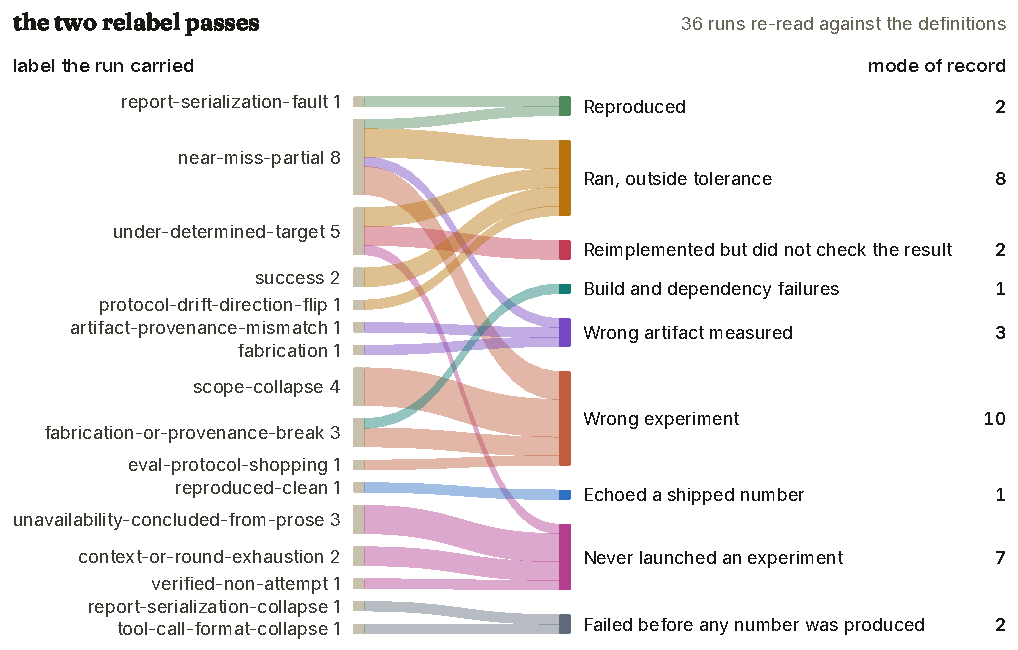
\includegraphics[width=\textwidth]{figures/app_G_relabel_flow}
\caption{The 36 runs the two relabel passes re-read, from the label each
carried to its mode of record, with ribbons in the color of the destination
mode and widths in runs.}
\label{fig:app-g-relabel-flow}
\end{figure}

\begin{figure}[htbp]
\centering
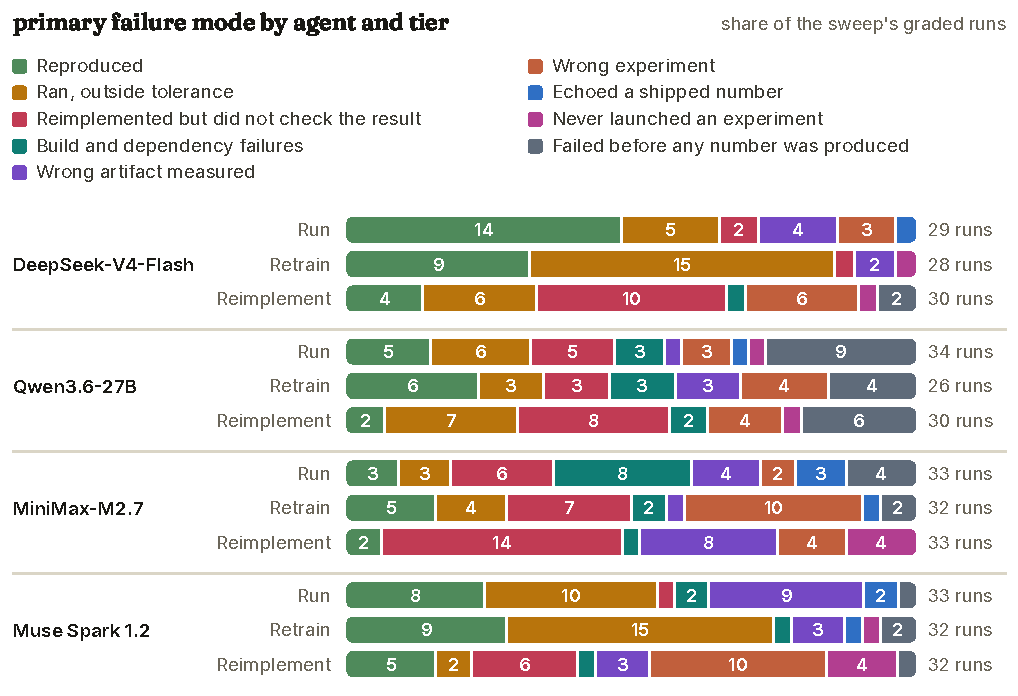
\includegraphics[width=\textwidth]{figures/app_G_agent_tier}
\caption{Primary failure mode by agent and tier over the 400 cells, each
bar normalized to its sweep's cells, in the order and colors of
Figure~\ref{fig:failure-modes}.}
\label{fig:app-g-agent-tier}
\end{figure}

\subsection{Failure modes of the frontier runs}
\label{app:frontier-modes}

To compare failures across the two sets of runs, Claude Sonnet 5 labeled the
main failure of each of the \todo{31} failing frontier runs
(Appendix~\ref{app:frontier}) from its transcript and the mode definitions of
Table~\ref{tab:taxonomy}, without seeing the verdict, the score, or the arm.
Table~\ref{tab:frontier-modes} sets the labels beside those of the 300 labeled
failing cells of the open agents. The three modes that report a number without
a valid measurement (Reimplemented but did not check the result, Wrong
artifact measured, and Echoed a shipped number) hold \todo{4 of 31} frontier
failures (13\%, 95\% interval 5\% to 29\%) against 110 of 300 (37\%, 31\% to
42\%) for the open agents, and the two modes that end without a number (Never
launched an experiment and Failed before any number was produced) hold
\todo{14 of 31} against 44 of 300 (15\%, 11\% to 19\%). The \todo{6} frontier
runs that never launched an experiment are all on 2505.16927 and 2503.14698,
two Reimplement papers on which the open agents also failed.
% src: results/frontier/failure_modes.csv; results/frontier/coder_calibration_groups.md; results/frontier/never_launched_check.md; moves with: the remaining frontier runs

Because the frontier labels come from a different coder than the labels of the
main results, we ran the same blind coder on 50 open-agent runs sampled across
the eight failing modes. It agrees with the paper's label on 28 of the 50
(Cohen's $\kappa = 0.48$), and reweighted to the mode sizes it puts the first
group at 46\% of open-agent failures (35\% to 58\%) and the second at 23\%
(14\% to 33\%), so the coder does not explain the lower share of the first
group in the frontier runs.
% src: results/frontier/coder_calibration.md (28 of 50, kappa 0.48); results/frontier/coder_calibration_groups.md (46.2%, 34.8 to 58.3; 22.8%, 14.4 to 33.3)

\begin{table}[ht]
\centering
\small
\begin{tabular}{@{}lrr@{}}
\toprule
Mode & Open agents (of 300) & Frontier runs (of \todo{31}) \\
\midrule
Ran, outside tolerance & 76 & \todo{5} \\
Reimplemented but did not check the result & 63 & \todo{3} \\
Wrong experiment & 46 & \todo{4} \\
Wrong artifact measured & 38 & \todo{1} \\
Failed before any number was produced & 31 & \todo{8} \\
Build and dependency failures & 24 & \todo{4} \\
Never launched an experiment & 13 & \todo{6} \\
Echoed a shipped number & 9 & \todo{0} \\
\bottomrule
\end{tabular}
\caption{Primary failure mode of the failing runs, open agents beside the
frontier runs.}
\label{tab:frontier-modes}
\end{table}

\subsection{Failure taxonomy examples}

For \texttt{reimplement-without-validating}, on paper 2510.08177~\citep{luo2025rebalancing} the agent
wrote its own version of the paper's baseline, scored it below the paper's
number for that baseline, and kept building on its version anyway.

\begin{agentturn}{Round 56, agent.\ Paper 2510.08177, MiniMax-M2.7, sweep 2936132.}
Best All: 40.82\% (ep 20)\\
Target (paper ProCo+MORE): 65.9\%\\
Paper CE baseline: 61.4\%\\
Our CE-only baseline: 54.21\%\\
Gap vs target: -25.08\%
\end{agentturn}

The third and fourth lines are the paper's baseline and the agent's copy of
it. The gap was still there at the end of the run.

For \texttt{scope-substitution}, on paper 2505.10039~\citep{chen2025circuit} the agent picked a
different arm from the pinned one at round 6, before writing any code, because
it was easier to implement. It never measured the pinned arm and reported the
number from the arm it chose.

\begin{agentturn}{Round 6, agent.\ Paper 2505.10039, DeepSeek-V4-Flash, sweep 2918306.}
The EAP method shows the largest gap and is the cleanest to implement (single forward/backward pass, no iterative search).
\end{agentturn}

Neither arm had released code, so both needed a port, and the agent chose
the easier one. Figure~\ref{fig:app-g-exit-by-mode} shows the rounds used and
the share of the grant spent at exit for every labeled run by mode.

\begin{figure}[htb]
\centering
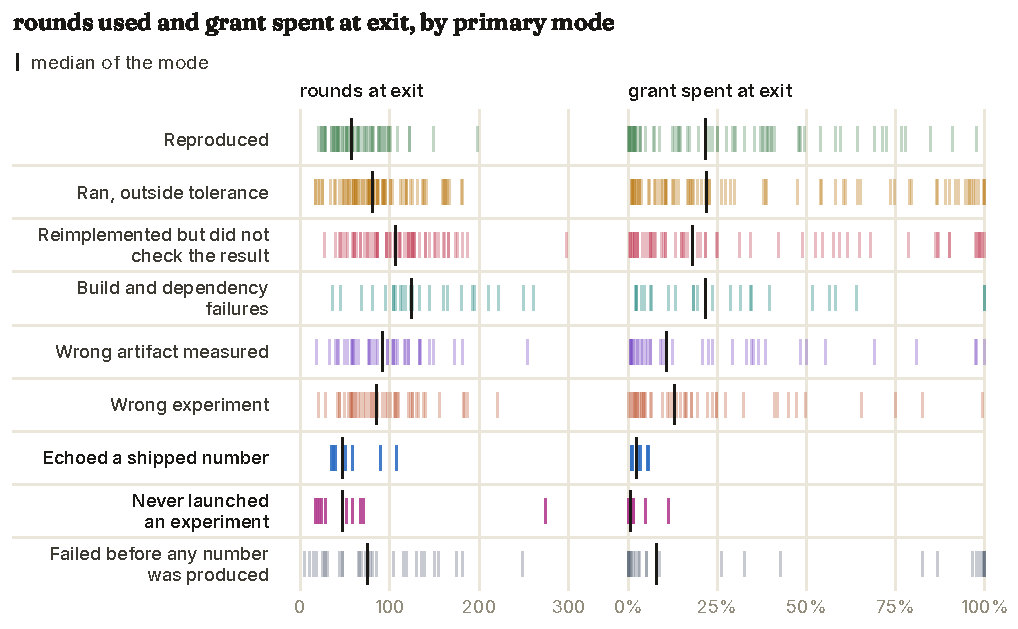
\includegraphics[width=\textwidth]{figures/app_G_exit_by_mode}
\caption{Rounds used and share of the H100 grant spent at exit, one tick per
labeled run, with each mode's median as a tick. Never launched an experiment
and Echoed a shipped number exit earliest.}
\label{fig:app-g-exit-by-mode}
\end{figure}

For \texttt{environment-fights}, on paper 2511.20906~\citep{chun2025dasip} an incompatible pair of
robosuite and mujoco versions silently broke the released dataset converter.
The agent had already trained on the broken output when it found the problem.

\begin{agentturn}{Round 233, agent.\ Paper 2511.20906, DeepSeek-V4-Flash, sweep 2918306.}
This is the smoking gun: **the saved abs dataset is broken** -{}- the abs actions don\textquotesingle t reproduce the expert trajectory even from the correct initial state.
\end{agentturn}

The defect is in the released code as it runs on this host, and the run
spent the rest of its budget on it.

\FloatBarrier  % Figure 20 prints above the Appendix H heading, so the first vignette fills its page
